\newcommand{\compable}[2]{#1 \circ #2 \downarrow}
\begin{frame}[fragile]
    \frametitle{Choice Algebra}

\textbf{Intuition:} Consider a judgement $\Gamma \vdash \phi$, the context constrians choices, the reachability property is existis a choice such that make a property $\phi$ hold.

\textbf{The Algebra should be able to express:}
\begin{itemize}
    \item Resource and separation: when there are multiple varaibles, if they are independent.
    \item Union: in coverage type we have ``merge rule''; in incorrectness logic we have ``disjunction rule'':
    \mprooftr{40mm}{
        $[P_1]C [Q_1] \quad[P_2]C [Q_2] $
       }{Disjunction}{
        $[P_1 \lor P_2]C [Q_1 \lor Q_2]$}
    \item These rule can deal with control flows in the reachability reasoning.
\end{itemize}

\textbf{Idea:} we introduce $\times$ operator (multiplication) and $+$ operator (addition) to express the separation product and union.

\end{frame}

\begin{frame}[fragile]
    \frametitle{Choice Algebra: Commutative Semiring}

\begin{definition}[Substitution and Carrier Set]
    A substitution $\sigma: \Code{Var} \rightharpoonup \Code{Value}$ is a partial function (mapping) from variables to resources. A element $m$ in carrier is a set of substitutions \textbf{share the same domain}, the carrier set is $\mathcal{M} = \mathcal{P}(\Code{Var} \rightharpoonup \Code{Value})$.
\end{definition}

\begin{definition}[Unit Element]
    The unit element of addition $\mathbf{0}$ is defined as empty set $\emptyset$; the unit element of multiplication $\mathbf{1}$ is defined as singleton set $\{\emptyset\}$.
\end{definition}

\begin{definition}[Addition and Multiplication] There are partial operations:
    \begin{itemize}
        \item $m_1 + m_2 \doteq m_1 \cup m_2$ when $\Dom{m_1} = \Dom{m_2}$.
        \item $m_1 \times m_2 \doteq \{ \sigma_1 \cup \sigma_2 ~|~ \sigma_1 \in m_1 \land \sigma_2 \in m_2 \}$ when $\Dom{m_1} \cap \Dom{m_2} = \emptyset$.
    \end{itemize}
\end{definition}
        
\end{frame}

\begin{frame}[fragile]
    \frametitle{Choice Algebra: Examples}

\begin{figure}
    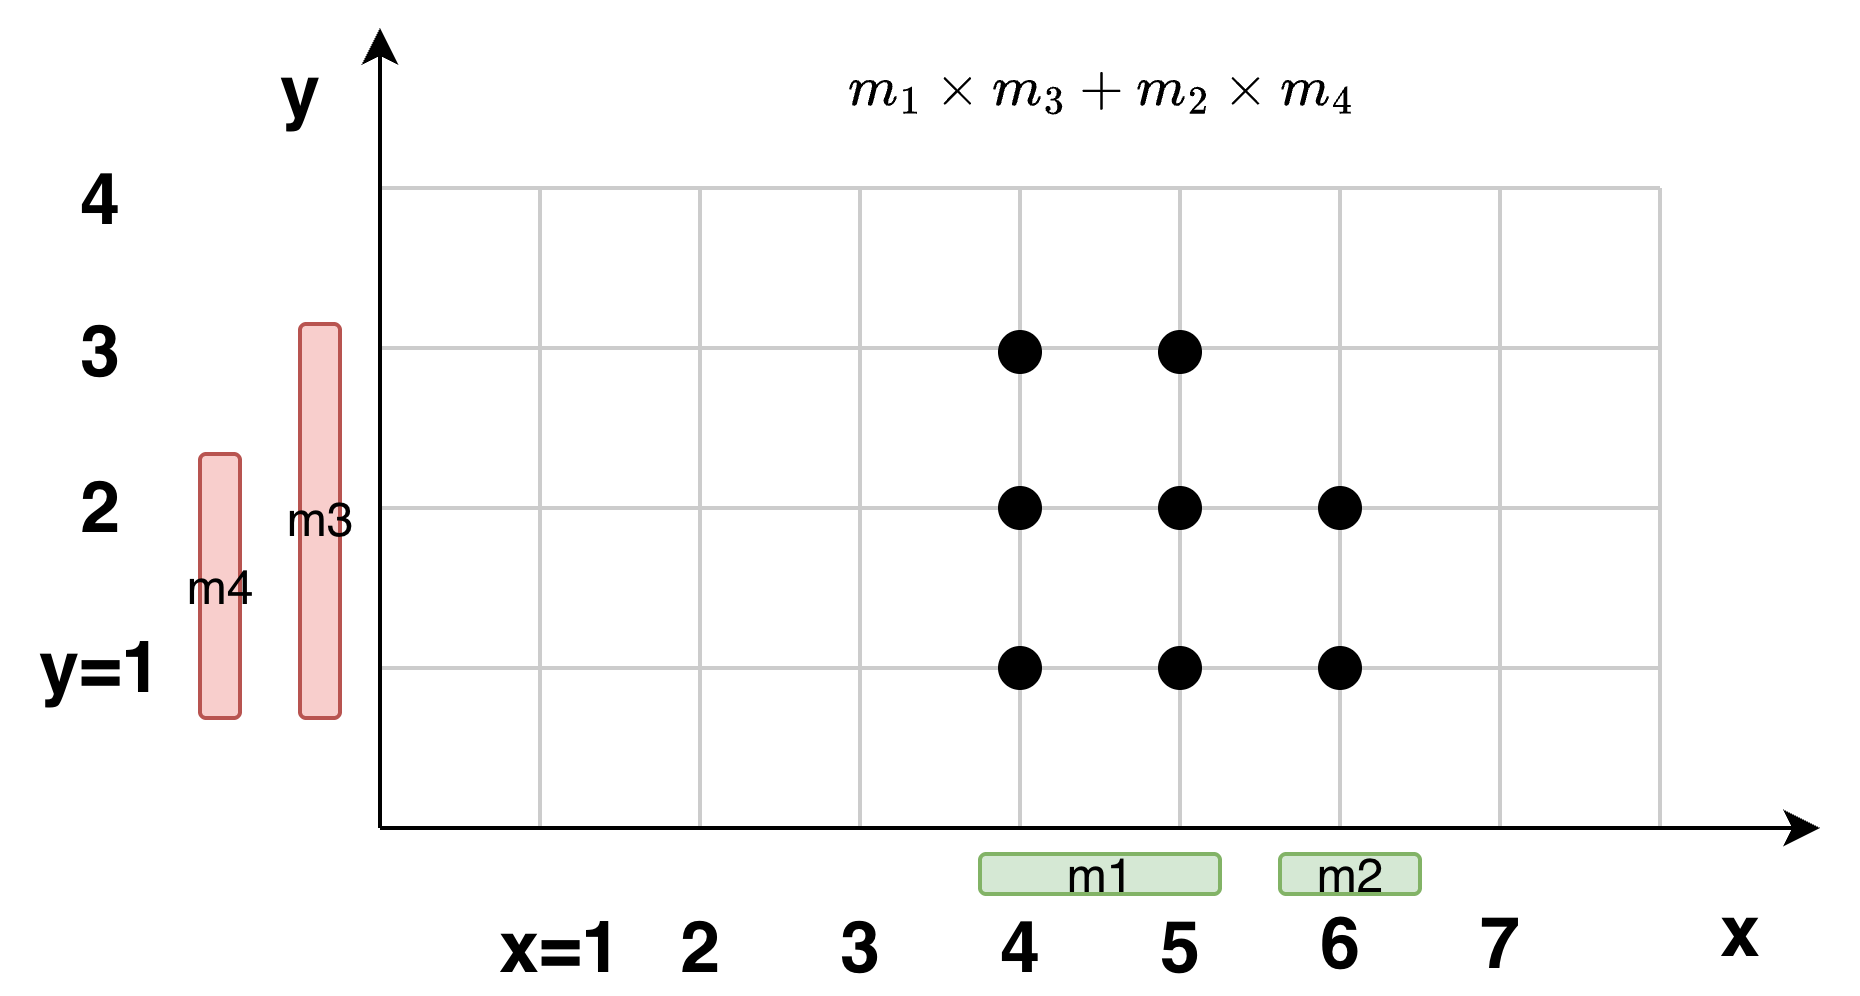
\includegraphics[width=0.8\textwidth]{figures/Ex1.drawio.png}
\end{figure}

\textbf{Example:} We show that how to use smaller resource to construct a larger resource; the atomic resource can be a ``line'' (e.g. $m_1$). Note that the ``shape'' does not need to be connected.

\textbf{Question:} How to define the partial order relation $\leq$?

\end{frame}

\begin{frame}[fragile]
    \frametitle{Choice Algebra: Partial Order}

\textbf{Intuition:} The partial order relation $\leq$ is ``entailment'' relation in the logic, where $a \leq b$ means $\forall \phi. a \models \phi \impl b \models \phi$.

% \textbf{Problem:} We have both over- and under- modality, and under- modality is contravariant.

\textbf{Intuition:} Assume $a\leq a + b$ since the $a + b$ contains ``more choices''. A reachability holds with smaller resource (choices) then also holds with larger resource.

\begin{figure}
    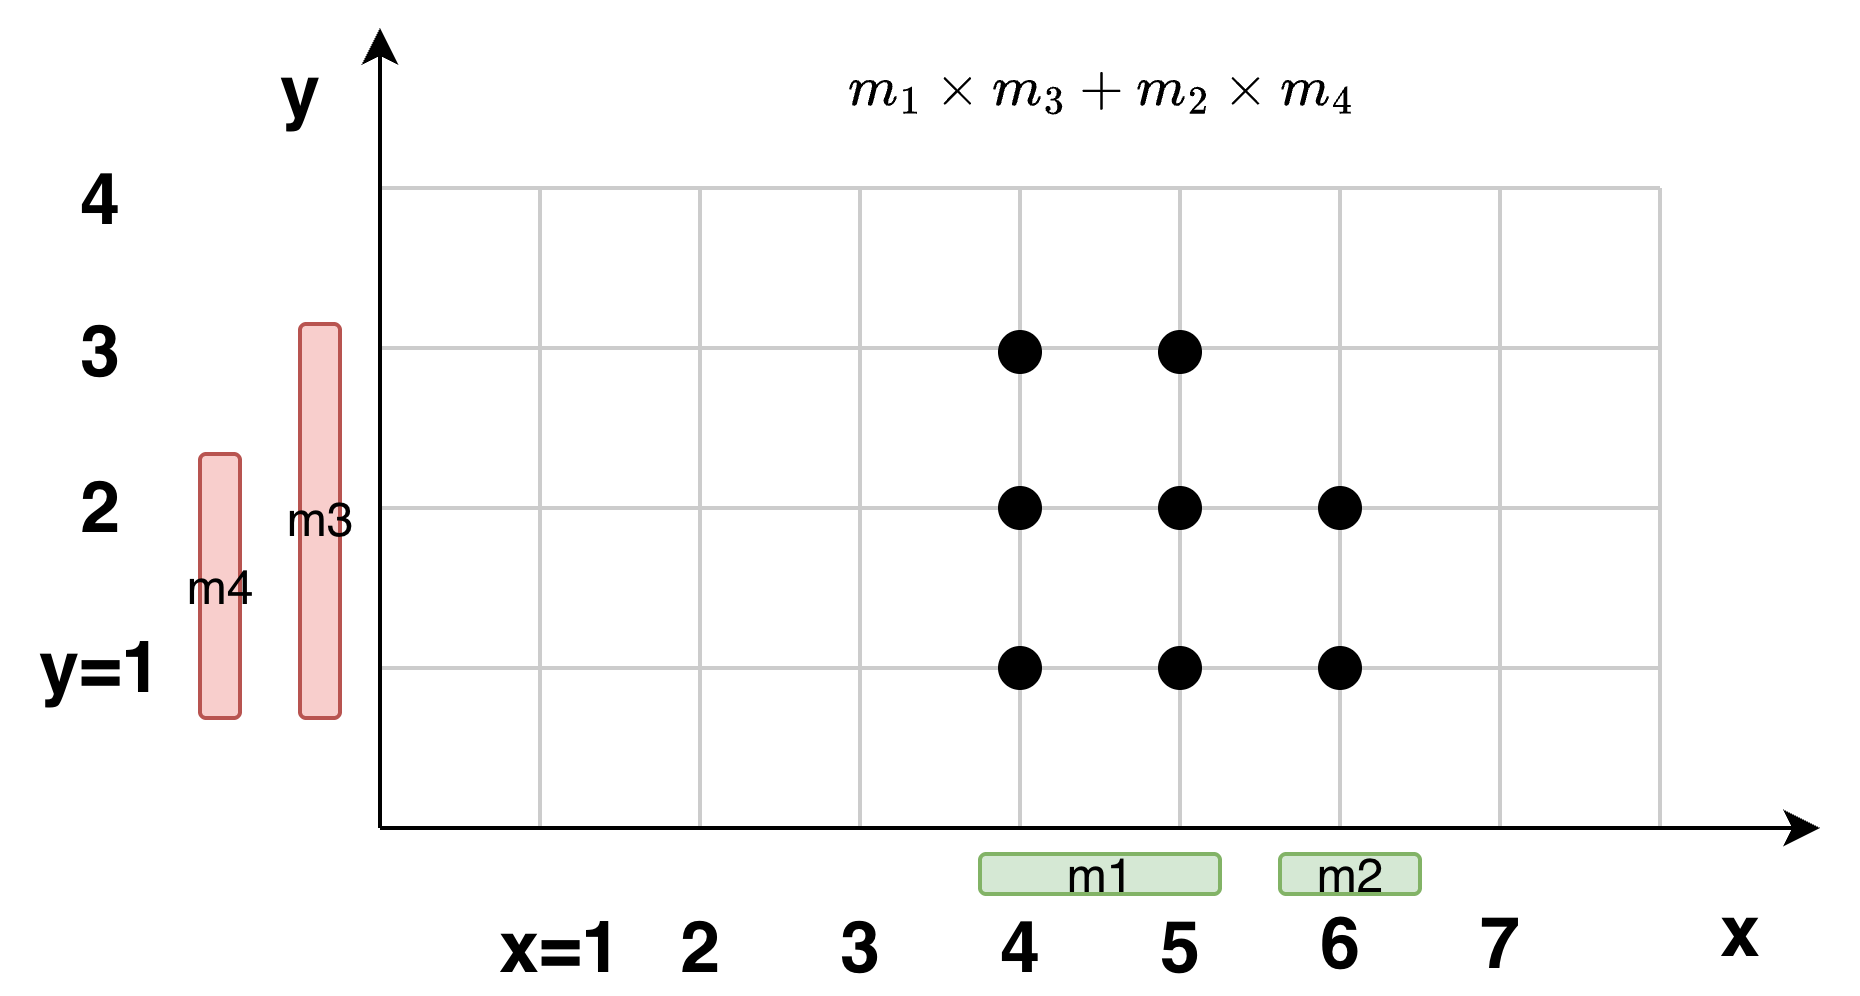
\includegraphics[width=0.8\textwidth]{figures/Ex1.drawio.png}
\end{figure}


\end{frame}

\begin{frame}[fragile]
    \frametitle{Choice Algebra: Partial Order}

\textbf{Question:} Compare $m_1$ with $m_1 \times m_2$?

\textbf{Intuition:} The $m_1 \times m_2$ can contains useless choices ($m_2$). 

\textbf{Observation:} If we have a set of choices $m_1 \times m_2$, we can projects thus choices into $\Dom{m_1}$ to recover $m_1$, the reverse is not true.

\textbf{Intuition:} $m_1 \leq m_1 \times m_2 + m_3$.

\begin{definition}[Partial Order]
    $m_1 \leq m_4$ iff $\exists m_2\;m_3. m_1 \times m_2 + m_3 = m_4$.
\end{definition}

\begin{lemma}[Bifunctoriality]
    $m_1 \leq m_2 \land m_3 \leq m_4 \impl m_1 \times m_3 \leq m_2 \times m_4$.
\end{lemma}

\end{frame}

\begin{frame}[fragile]
    \frametitle{Choice Logic}

\begin{definition}[Choice Logic] A choice logic is an intuitive logic with $*$, $\wand$, and $\oplus$ operators.
\end{definition}
\begin{itemize}
    \item $m \models \phi * \psi$ iff $\exists m_1\; m_2. m_1 \times m_2 \leq m \text{ and } m_1 \models \phi \text{ and } m_2 \models \psi$.
    \item $m \models \phi \wand \psi$ iff $\forall m'. m' \models \phi  \impl m' \times m \models \psi$.
    \item $m \models \phi \oplus \psi$ iff $\exists m_1, m_2. m_1 + m_2 \leq m \text{ and } m_1 \models \phi \text{ and } m_2 \models \psi$.
    \item $m \models P$ iff $\exists \sigma \in m. \sigma(P)$.
    \item $m \models \true$ always; $m \models \false$ never.
    \item We write $\models \phi$ when $\textbf{1} \models \phi$ holds (note that $\textbf{0}$ cannot model any proposition).
\end{itemize}

\begin{definition}[Underapproximation Modality]
    \begin{itemize}
        \item $m \models \boxtimes_5 \phi$ iff $\{\sigma ~|~ \{\sigma\} \models \phi \land \Dom{\sigma} = \Code{FV}(\phi) \} \leq m$.
    \end{itemize}
\end{definition}

\begin{definition}[Entailment]
    $\phi \models \psi$ holds, if for all $m$, $m \models \phi$ implies $m \models \psi$.
\end{definition}

\end{frame}

\begin{frame}[fragile]
    \frametitle{Choice Logic: Monotonicity}

    \begin{lemma}[Merge rule]
        $m \models \boxtimes_5 P_1 \oplus \boxtimes_5 P_2$ iff $m \models \boxtimes_5 (P_1 \lor P_2)$.
    \end{lemma}


\begin{lemma}[Kripke's Monotonicity]
        $m \leq m'$ and $m \models \phi$ implies $m' \models \phi$.
\end{lemma}

\begin{lemma}[Overapproximation]
    $\models P \impl Q$ holds, and $m \models P$ then $m \models Q$.
\end{lemma}

\begin{lemma}[Underapproximation]
    $\models P \impl Q$ holds, and $m \models \boxtimes_5 Q$ then $m \models \boxtimes_5 P$.
\end{lemma}

\end{frame}

\begin{frame}[fragile]
    \frametitle{Choice Logic: Examples}

    \begin{figure}
        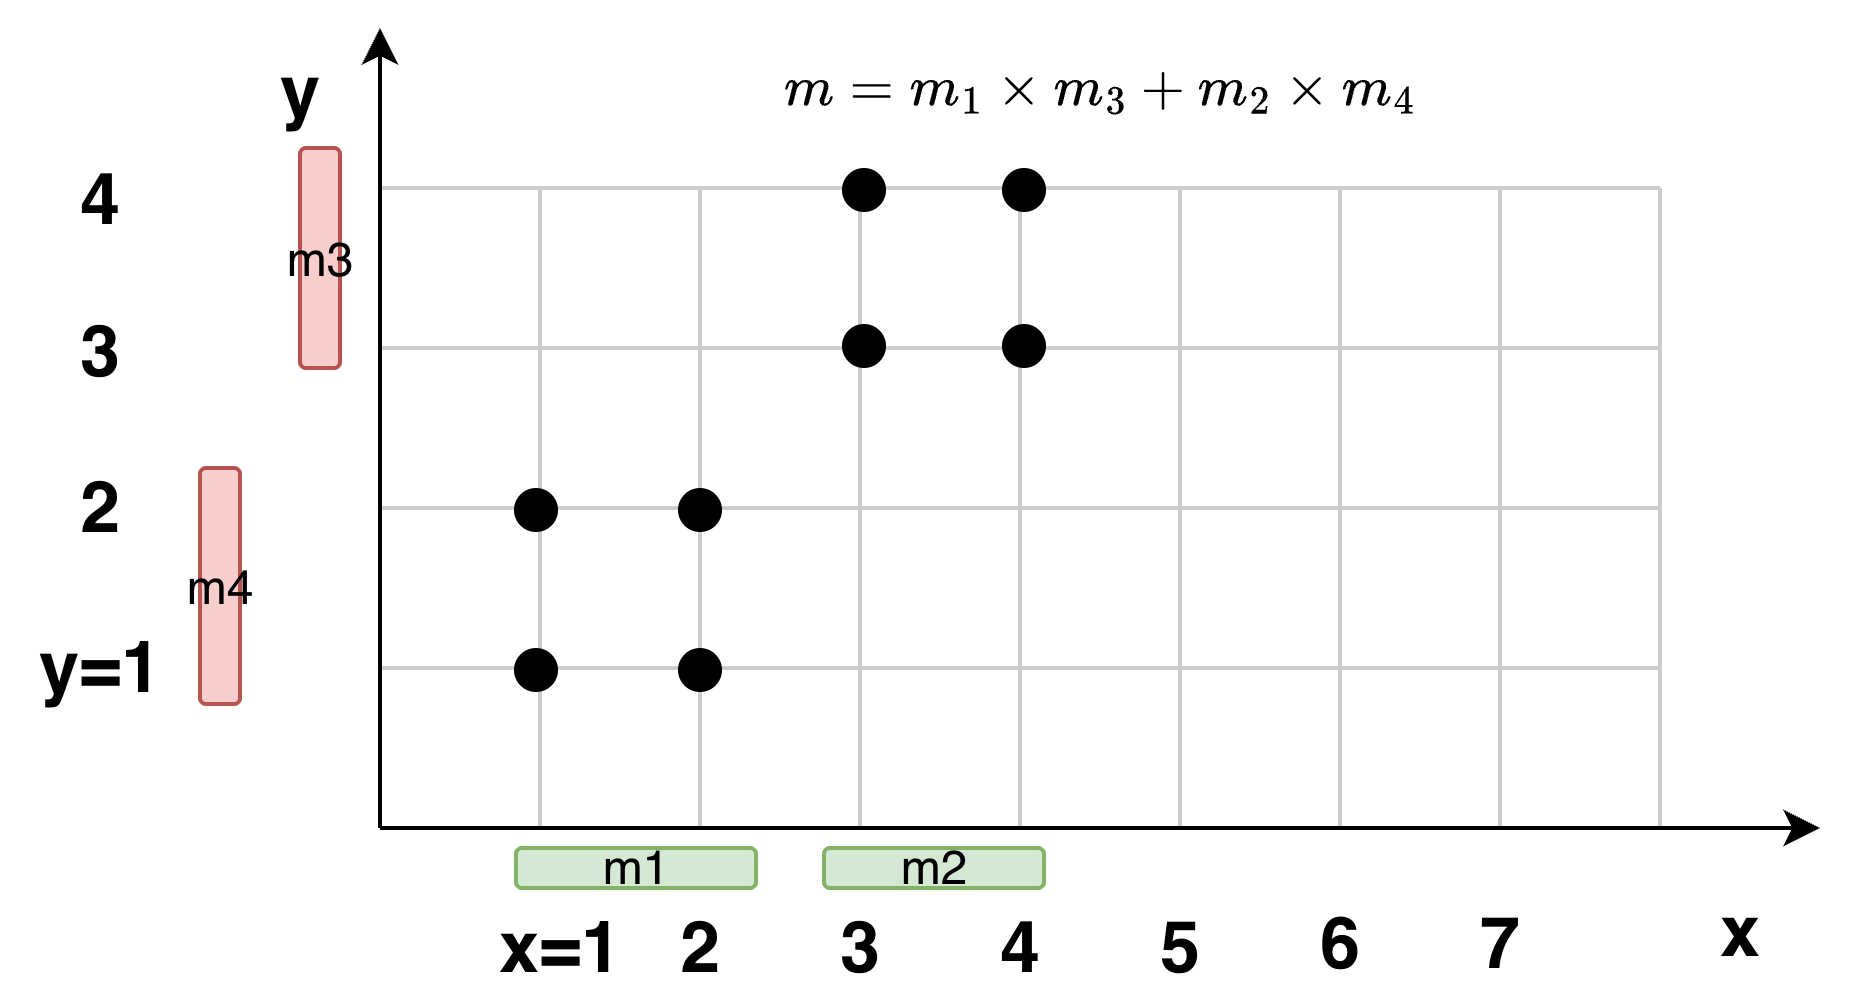
\includegraphics[width=0.8\textwidth]{figures/Ex2.drawio.png}
    \end{figure}

\textbf{Example:} We show that $m \models \boxtimes_5 (1 \leq x \leq 4)$.
\begin{itemize}
    \item $m_1 \times m_3 \leq m_1 \models \boxtimes_5 (1 \leq x \leq 2)$ by definition of $\boxtimes_5$.
    \item $m_2 \times m_4 \leq m_2 \models \boxtimes_5 (3 \leq x \leq 4)$ by definition of $\boxtimes_5$.
    \item $m \models \boxtimes_5 (1 \leq x \leq 2) \oplus \boxtimes_5 (3 \leq x \leq 4)$ by definition of $\oplus$.
    \item $m \models \boxtimes_5 (1 \leq x \leq 4)$ by merge rule. 
\end{itemize}
\end{frame}

\begin{frame}[fragile]
    \frametitle{Choice Logic: Examples}

    \begin{figure}
        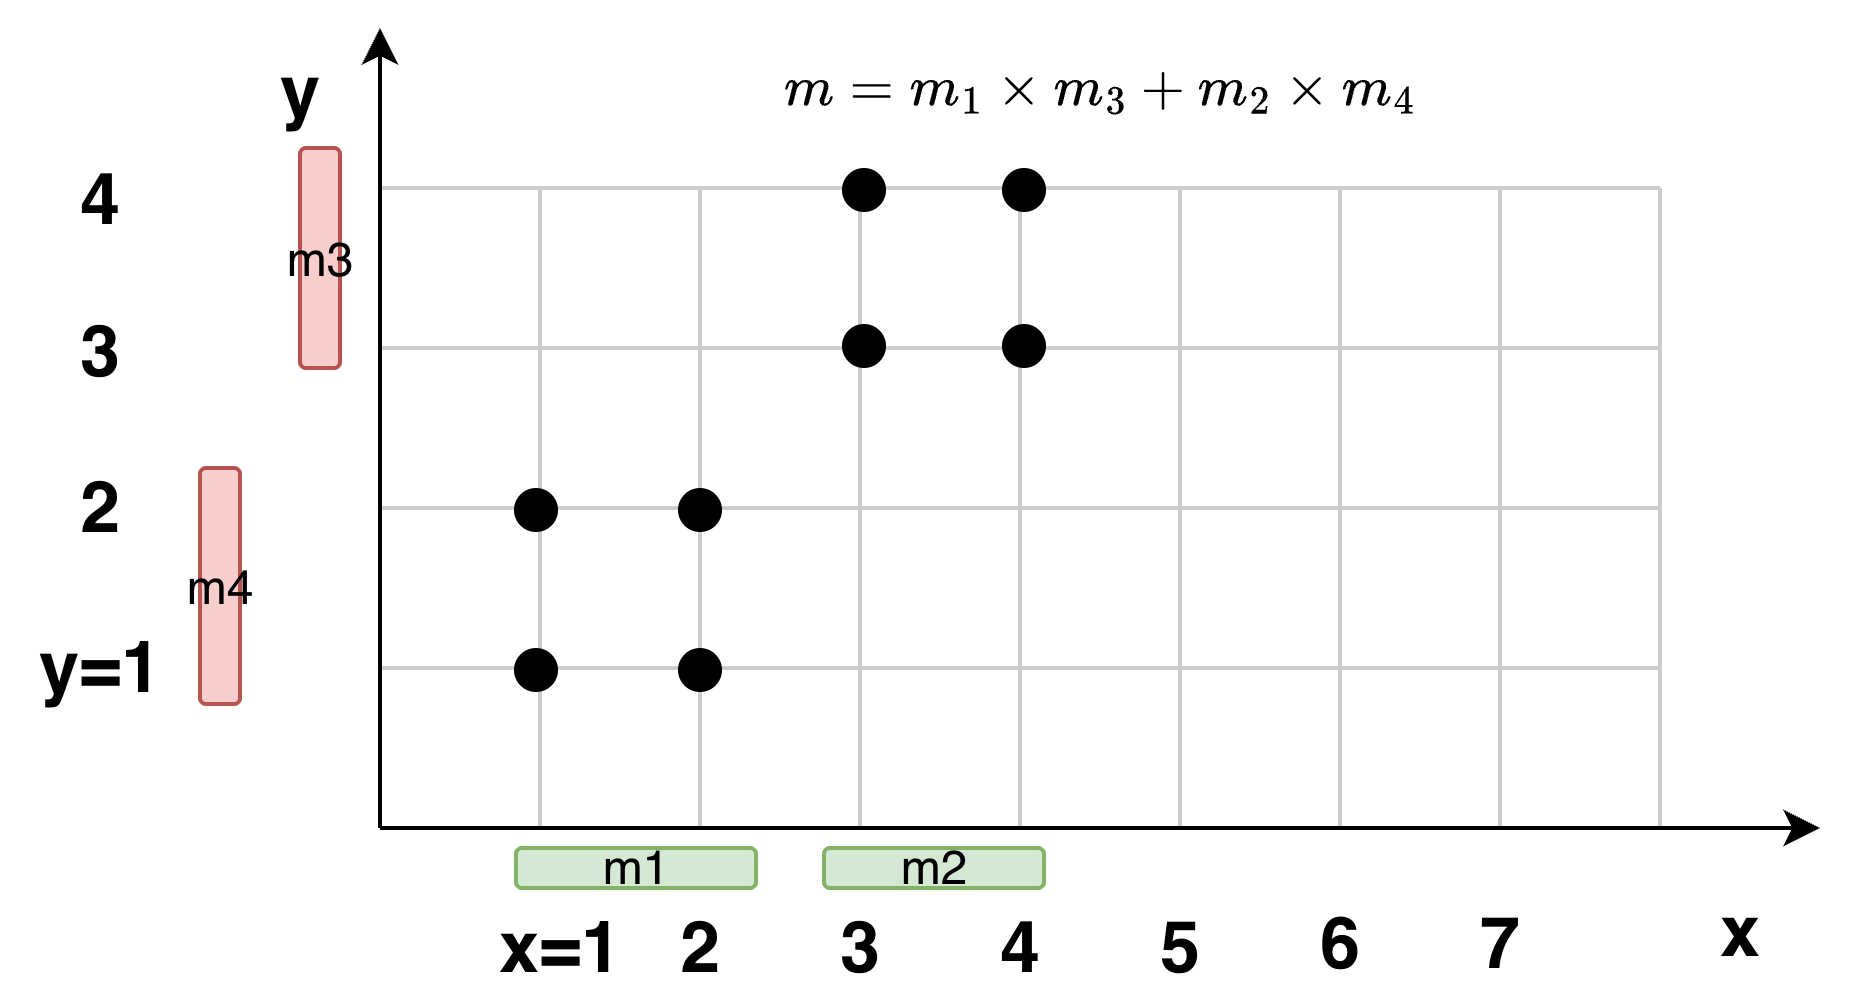
\includegraphics[width=0.6\textwidth]{figures/Ex2.drawio.png}
    \end{figure}

\textbf{Intuition:} If we don't have $\oplus$ operator, we cannot prove it!
\begin{itemize}
    \item Notice that $m$ which has domain $\{x,y\}$ however the property has domain $\{x\}$. Thus we need docompose $m$ into a form $m_x \times m_y$ (a rectangle).
    \item However, we cannot find a rectangle $\leq m$ and still can cover $1 \leq x \leq 4$. 
    \item The $+$ allows us to use the ``reminder'' after decomposition.
\end{itemize}
\end{frame}

\begin{frame}[fragile]
    \frametitle{Choice Logic: compare with previous version}

\begin{figure}
    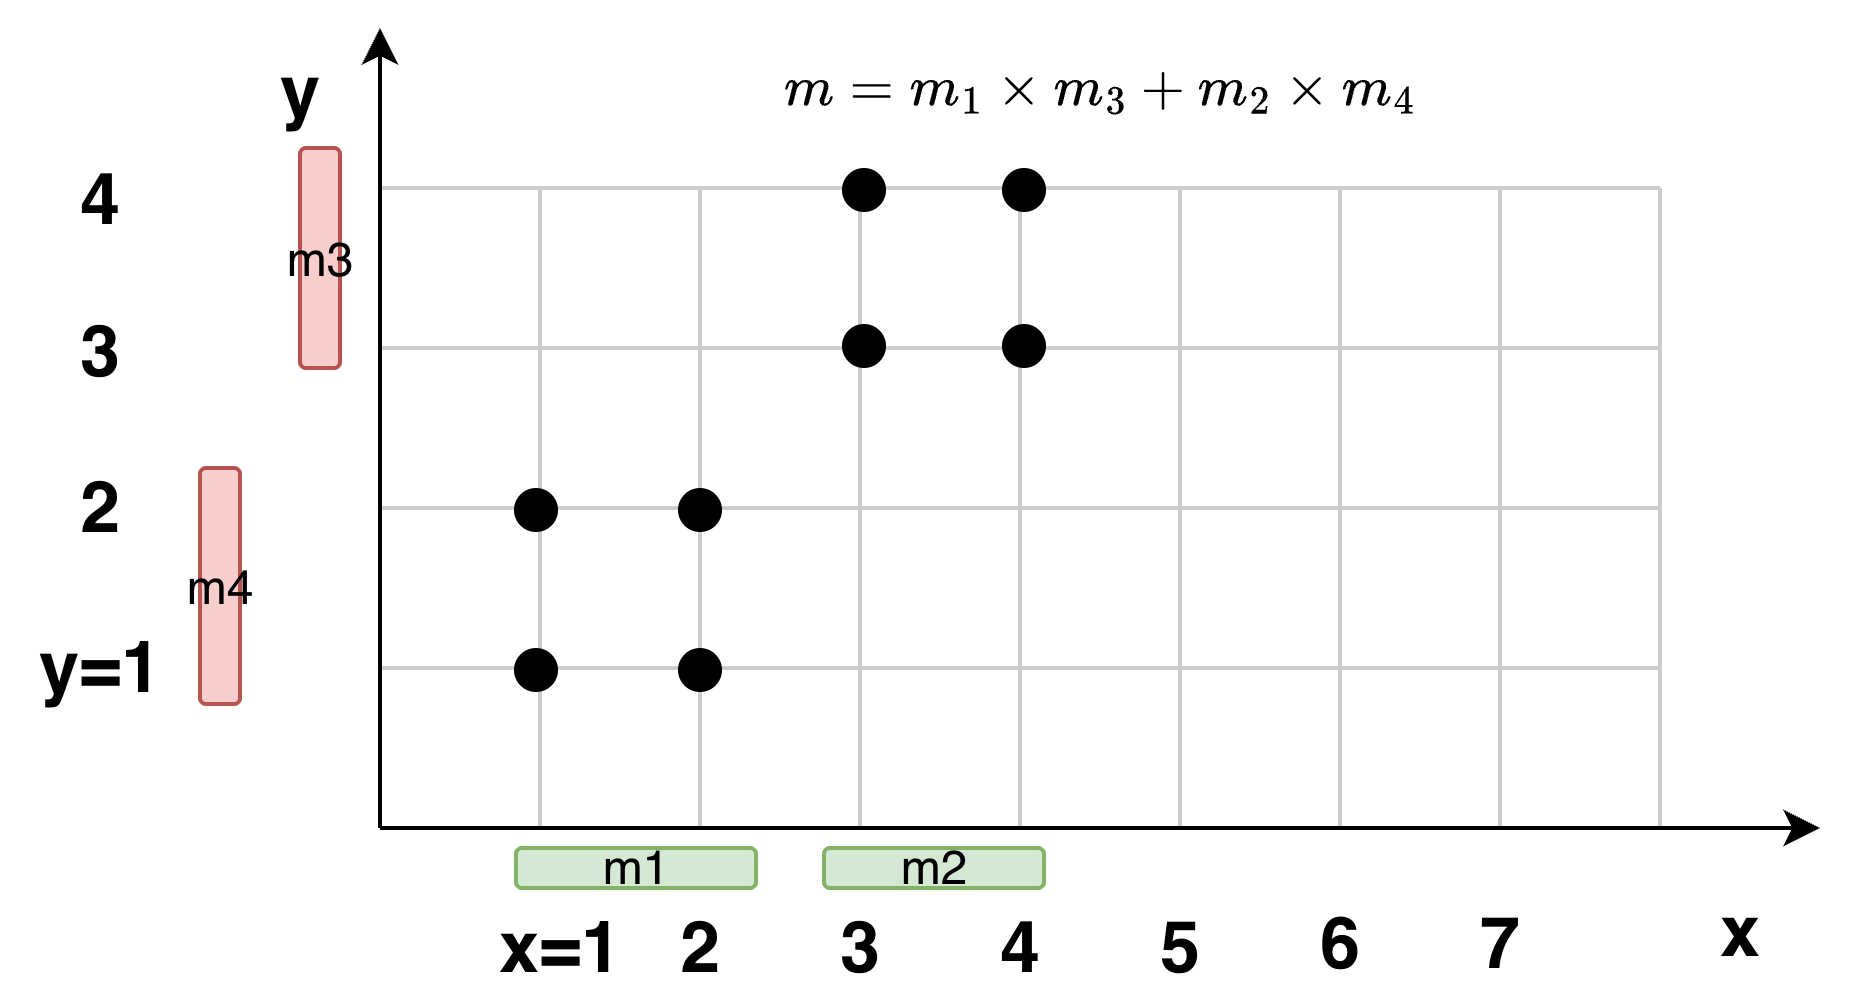
\includegraphics[width=0.6\textwidth]{figures/Ex2.drawio.png}
\end{figure}

\textbf{Version 1: model} We build a whole model to record the relation of choices, i.e., we record $m$, $m_1$, $m_2$, $m_3$, $m_4$, $m_1 + m_2$, $m_3 + m_4$, and their relations.
\begin{itemize}
    \item Each time we talk about $m_3$, we still remember $m$.
    \item Thus we know $m_3 \times m_2$ is valid (since $m_3 \times m_2 \leq m$).
    \item We also know $(m_1 + m_2) \times (m_3 + m_4)$ is invalid.
    \item We also don't have $+$ operator, since the model contains all valid sums.
\end{itemize}
\end{frame}

\begin{frame}[fragile]
    \frametitle{Choice Logic: compare with previous version}

\begin{figure}
    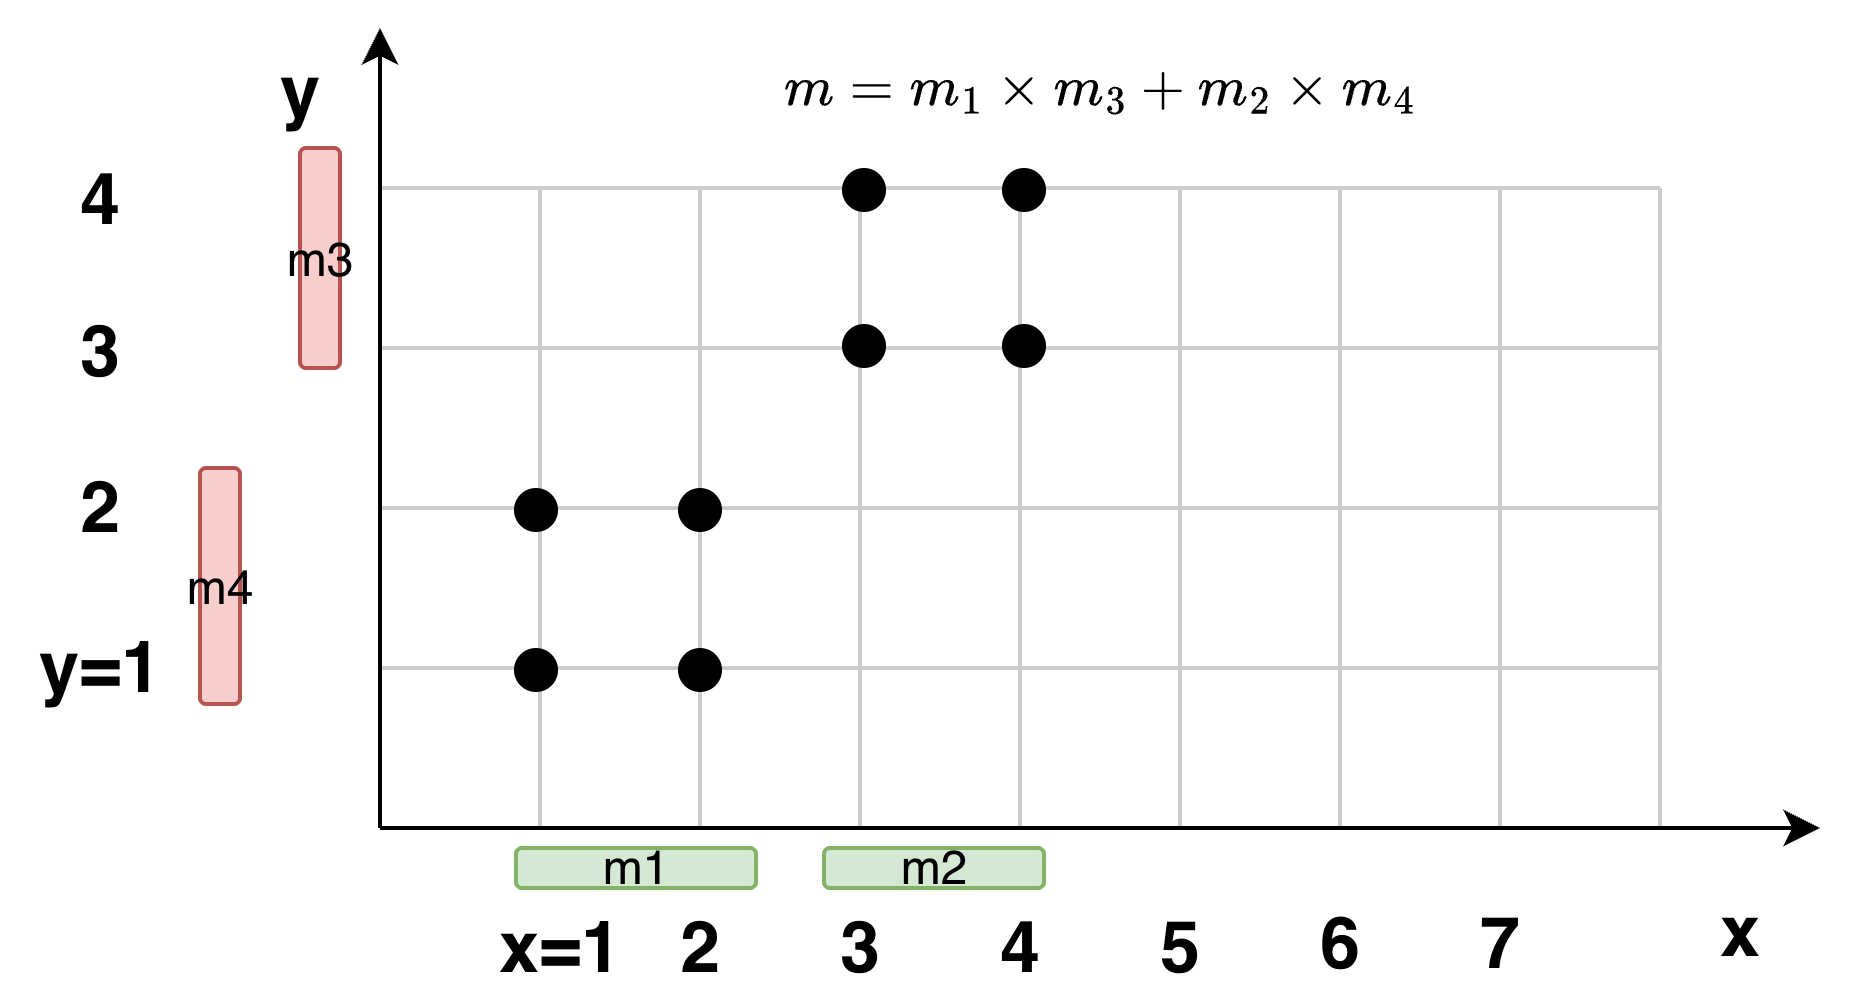
\includegraphics[width=0.6\textwidth]{figures/Ex2.drawio.png}
\end{figure}

\textbf{Version 1: $(\Sigma^+, \Sigma^-)$} We build a whole model to record the relation of choices, i.e., we record $m$, $m_1$, $m_2$, $m_3$, $m_4$, $m_1 + m_2$, $m_3 + m_4$, and their relations.
\begin{itemize}
    \item Each time we talk about $m_3$, we still remember $m$.
    \item Thus we know $m_3 \times m_2$ is valid (since $m_3 \times m_2 \leq m$).
    \item We also know $(m_1 + m_2) \times (m_3 + m_4)$ is invalid.
    \item We also don't have $+$ operator, since the model contains all valid sums.
\end{itemize}
\end{frame}

\begin{frame}[fragile]
    \frametitle{Choice Logic: compare with previous version}

\begin{figure}
    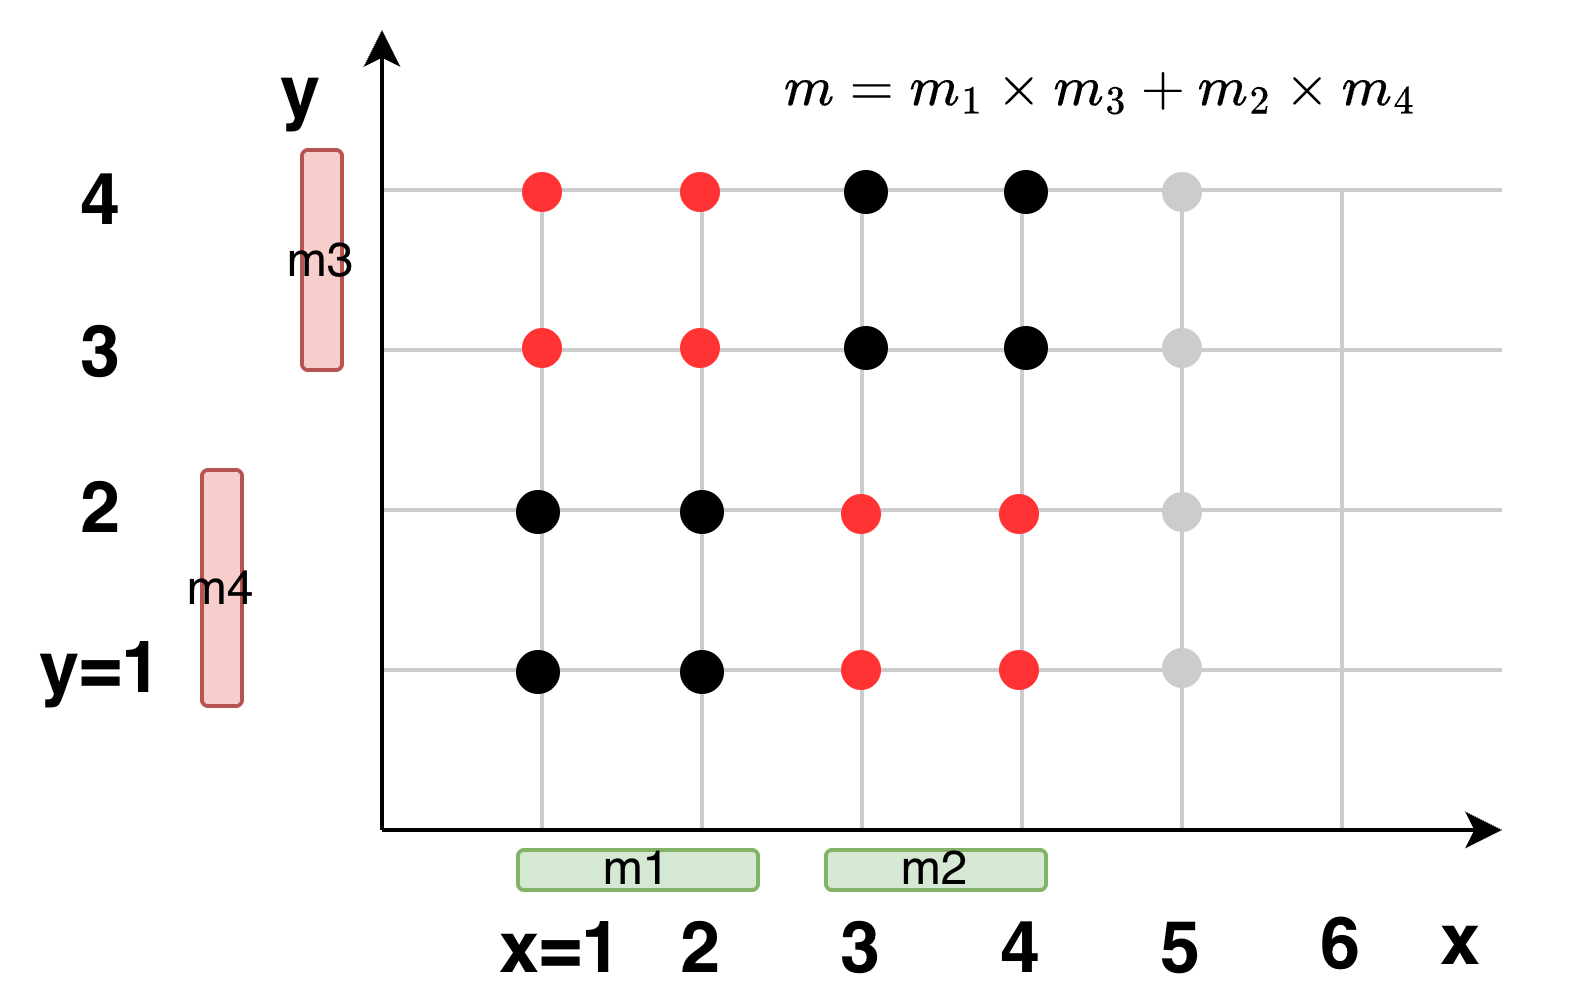
\includegraphics[width=0.6\textwidth]{figures/Ex3.drawio.png}
\end{figure}

\textbf{Version 2: $(\Sigma^+, \Sigma^-)$} we express $m$ as a set positive set (black points) and negative set (red points).
\begin{itemize}
    \item The red nodes are ``disallowed choices'', thus we can always track them -- even in $m_3$ that has a different domain.
    \item $m_1 \times m_3$ is empty since all choices are cancelled out by the red nodes.
    \item Gray points are nagtive but can be ignored, since they are never used.
\end{itemize}
\end{frame}

\begin{frame}[fragile]
    \frametitle{Choice Logic: compare with previous version}

\textbf{Problem:} All complex definition in previous version come from we want to use single resource to track knowledge even out of its domain.

\textbf{Intuition:} We don't want to lose information (e.g., negative choices), however we don't know where to store them since $\leq$ relation always drop information.

\textbf{Idea:} We introduce $m = m_1 \times m_2 + m_3$, where $m_1 \times m_2 \leq m$ indeed lose the information $m_3$, but the $+$ allows us to reuse this reminder.

\mprooftr{50mm}{
 $m_1 \times m_2 \models \boxtimes_5 \phi_1$ \quad $m_3 \models \boxtimes_5 \phi_2$
}{Merge rule}{
 $m_1 \times m_2 + m_3 \models \boxtimes_5 (\phi_1 \lor \phi_2)$}

\end{frame}

\begin{frame}[fragile]
    \frametitle{Choice Logic: Persistency}

\textbf{Idea:} Persistent proposition $\phi$ means $\phi$ holds without exclusive ownership; persistent proposition can be duplicated: $\phi * \phi \iff \phi$.

\textbf{Intuition:} We know that pure proposition $P$ is persistent, and singleton coverage is also persistent.

\textbf{Problem:} $\boxtimes_5 (x = 1) * \boxtimes_5 (x = 1)$ is not well-formed.

\begin{definition}[Addition and Multiplication] There are partial operations:
    \begin{itemize}
        \item $m_1 + m_2 \doteq m_1 \cup m_2$ when $\Dom{m_1} = \Dom{m_2}$.
        \item $m_1 \times m_2 \doteq \{ \sigma_1 \cup \sigma_2 ~|~ \sigma_1 \in m_1 \land \sigma_2 \in m_2 \}$
        \item when $\forall \sigma_1 \in m_1, \forall \sigma_2 \in m_2. \forall x. x \in \Dom{\sigma_1} \land x \in \Dom{\sigma_2} \implies \sigma_1(x) = \sigma_2(x)$.
    \end{itemize}
\end{definition}

\begin{lemma}[Idempotency] $|m| \leq 2$ implies $m \times m = m$.
\end{lemma}

\end{frame}

\begin{frame}[fragile]
    \frametitle{Choice Logic: Persistency}

\begin{definition}[Persistency]
    \begin{itemize}
        \item $m \models \Box \phi$ iff there exists a singleton resource $m'$ (i.e., $|m'| = 1$) such that $m' \leq m$ and $m' \models \phi$.
    \end{itemize}
\end{definition}

\textbf{Intuition:} We ensure that there is no choice to be made.

\textbf{Note:} The resource $\textbf{0}$ cannot model any proposition; thus, we do not consider it.

\begin{lemma}[Persistence Elimination] $m \models \Box \phi$ implies $m \models \phi$.
\end{lemma}

\begin{lemma}[Persistence Duplicatable] $m \models \Box \phi$ implies $m \models \Box \phi * \Box \phi$.
\end{lemma}

\end{frame}

\begin{frame}[fragile]
    \frametitle{Choice Logic: Persistency}

\begin{lemma}[Persistence Pure] A pure proposition $P$ is persistent: $P \models \Box P$.
\end{lemma}
\begin{proof} A valid pure proposition holds under $\textbf{1}$. 
\end{proof}

\begin{lemma}[Persistence Idempotency] $\Box \phi \models \Box \Box \phi$.
\end{lemma}

\begin{lemma}[Persistence Conjunction] $\Box \phi_1 \land \phi_2 \models \Box \phi_1 * \phi_2$.
\end{lemma}
\begin{proof} Note that if a singleton resource $m' \leq m$, then we actually have $m' \times m = m$. This rule is not a part of standard $!$ modality in linear logic.
\end{proof}

\end{frame}


\begin{frame}[fragile]
    \frametitle{Choice Logic: Other modalities}

\begin{definition}[Modality]
    \begin{itemize}
        \item $m \models \diamond_5 \phi$ iff $\exists \sigma \in m. \{\sigma\} \models \phi$.
        \item \textbf{Note:} the persistency modality $\Box$ is exactly the possibility modality $\diamond_5$ in S5.
        \item $m \models \Box_5 \phi$ iff $\forall \sigma \in m. \{\sigma\} \models \phi$.
        \item Break the Kripke's Monotonicity: More resource doesn't mean still correct.
    \end{itemize}
\end{definition}

\textbf{Note:} The $\diamond_5$ modality works like ``overapproximation'' and $\boxtimes_5$ modality works like ``underapproximation''.

\textbf{Example:} Consider type context $x{:}\ort{\Int}{\vnu > 0}, y{:}\urt{\Int}{\vnu > 0}: \vdash ...$
\begin{itemize}
    \item can be expressed as $\diamond_5 (x > 0) \land \boxtimes_5 (y > 0) \models ...$.
    \item can also be expressed as $\diamond_5 (x > 0) * \boxtimes_5 (y > 0) \models ...$ (persistence conjunction rule)
    \item Overapproximation is presistency.
\end{itemize}
\end{frame}